\documentclass[twoside]{book}

% Packages required by doxygen
\usepackage{fixltx2e}
\usepackage{calc}
\usepackage{doxygen}
\usepackage[export]{adjustbox} % also loads graphicx
\usepackage{graphicx}
\usepackage[utf8]{inputenc}
\usepackage{makeidx}
\usepackage{multicol}
\usepackage{multirow}
\PassOptionsToPackage{warn}{textcomp}
\usepackage{textcomp}
\usepackage[nointegrals]{wasysym}
\usepackage[table]{xcolor}

% Font selection
\usepackage[T1]{fontenc}
\usepackage[scaled=.90]{helvet}
\usepackage{courier}
\usepackage{amssymb}
\usepackage{sectsty}
\renewcommand{\familydefault}{\sfdefault}
\allsectionsfont{%
  \fontseries{bc}\selectfont%
  \color{darkgray}%
}
\renewcommand{\DoxyLabelFont}{%
  \fontseries{bc}\selectfont%
  \color{darkgray}%
}
\newcommand{\+}{\discretionary{\mbox{\scriptsize$\hookleftarrow$}}{}{}}

% Page & text layout
\usepackage{geometry}
\geometry{%
  a4paper,%
  top=2.5cm,%
  bottom=2.5cm,%
  left=2.5cm,%
  right=2.5cm%
}
\tolerance=750
\hfuzz=15pt
\hbadness=750
\setlength{\emergencystretch}{15pt}
\setlength{\parindent}{0cm}
\setlength{\parskip}{3ex plus 2ex minus 2ex}
\makeatletter
\renewcommand{\paragraph}{%
  \@startsection{paragraph}{4}{0ex}{-1.0ex}{1.0ex}{%
    \normalfont\normalsize\bfseries\SS@parafont%
  }%
}
\renewcommand{\subparagraph}{%
  \@startsection{subparagraph}{5}{0ex}{-1.0ex}{1.0ex}{%
    \normalfont\normalsize\bfseries\SS@subparafont%
  }%
}
\makeatother

% Headers & footers
\usepackage{fancyhdr}
\pagestyle{fancyplain}
\fancyhead[LE]{\fancyplain{}{\bfseries\thepage}}
\fancyhead[CE]{\fancyplain{}{}}
\fancyhead[RE]{\fancyplain{}{\bfseries\leftmark}}
\fancyhead[LO]{\fancyplain{}{\bfseries\rightmark}}
\fancyhead[CO]{\fancyplain{}{}}
\fancyhead[RO]{\fancyplain{}{\bfseries\thepage}}
\fancyfoot[LE]{\fancyplain{}{}}
\fancyfoot[CE]{\fancyplain{}{}}
\fancyfoot[RE]{\fancyplain{}{\bfseries\scriptsize Generated by Doxygen }}
\fancyfoot[LO]{\fancyplain{}{\bfseries\scriptsize Generated by Doxygen }}
\fancyfoot[CO]{\fancyplain{}{}}
\fancyfoot[RO]{\fancyplain{}{}}
\renewcommand{\footrulewidth}{0.4pt}
\renewcommand{\chaptermark}[1]{%
  \markboth{#1}{}%
}
\renewcommand{\sectionmark}[1]{%
  \markright{\thesection\ #1}%
}

% Indices & bibliography
\usepackage{natbib}
\usepackage[titles]{tocloft}
\setcounter{tocdepth}{3}
\setcounter{secnumdepth}{5}
\makeindex

% Hyperlinks (required, but should be loaded last)
\usepackage{ifpdf}
\ifpdf
  \usepackage[pdftex,pagebackref=true]{hyperref}
\else
  \usepackage[ps2pdf,pagebackref=true]{hyperref}
\fi
\hypersetup{%
  colorlinks=true,%
  linkcolor=blue,%
  citecolor=blue,%
  unicode%
}

% Custom commands
\newcommand{\clearemptydoublepage}{%
  \newpage{\pagestyle{empty}\cleardoublepage}%
}

\usepackage{caption}
\captionsetup{labelsep=space,justification=centering,font={bf},singlelinecheck=off,skip=4pt,position=top}

%===== C O N T E N T S =====

\begin{document}

% Titlepage & ToC
\hypersetup{pageanchor=false,
             bookmarksnumbered=true,
             pdfencoding=unicode
            }
\pagenumbering{roman}
\begin{titlepage}
\vspace*{7cm}
\begin{center}%
{\Large Efficio Runtime C++ \\[1ex]\large 0.\+0.\+0.\+1 }\\
\vspace*{1cm}
{\large Generated by Doxygen 1.8.11}\\
\end{center}
\end{titlepage}
\clearemptydoublepage
\tableofcontents
\clearemptydoublepage
\pagenumbering{arabic}
\hypersetup{pageanchor=true}

%--- Begin generated contents ---
\chapter{Efficio Runtime for C++}
\label{index}\hypertarget{index}{}\section*{Efficio\+C\+PP}

Experimentation with Efficio in C++

\subsection*{For Developers }

The Efficio Runtime project automatically documents itself in a post-\/build step using \href{http://doxygen.org/}{\tt Doxygen}. To take advantage of the documenting feature, simply add the doxygen executables to the Windows P\+A\+TH environment variable. The current documentation can be found \href{https://htmlpreview.github.io/?https://raw.githubusercontent.com/Abantech/EfficioCPP/master/EfficioRuntime/doc/html/index.html}{\tt here} 
\chapter{R\+E\+A\+D\+ME}
\label{md_README}
\hypertarget{md_README}{}
\#\+Efficio C++ The Efficio C++ project is the base on which all other language projects are built.

\section*{Getting the Project to Build in Visual Studio }


\begin{DoxyEnumerate}
\item Download \href{http://swig.org/download}{\tt S\+W\+IG} for Windows v3.\+0.\+10.
\end{DoxyEnumerate}
\begin{DoxyEnumerate}
\item Add S\+W\+IG to the Path environment variable.
\end{DoxyEnumerate}
\begin{DoxyEnumerate}
\item Download \href{http://doxygen.org}{\tt Doxygen}.
\end{DoxyEnumerate}
\begin{DoxyEnumerate}
\item Add Doxygen to the Path environment variable.
\end{DoxyEnumerate}
\begin{DoxyEnumerate}
\item Download the Leap Motion S\+DK.
\end{DoxyEnumerate}
\begin{DoxyEnumerate}
\item Create an environment variable called L\+E\+A\+P\+\_\+\+S\+DK pointing to the Leap Motion S\+DK.
\end{DoxyEnumerate}
\begin{DoxyEnumerate}
\item When the project is compiled .cxx files will be generated or overwritten for each given target language. Make sure these are writable and if generated for the first time, are included in the vcxproj 
\end{DoxyEnumerate}
\chapter{Hierarchical Index}
\section{Class Hierarchy}
This inheritance list is sorted roughly, but not completely, alphabetically\+:\begin{DoxyCompactList}
\item \contentsline{section}{Efficio\+:\+:Body}{\pageref{class_efficio_1_1_body}}{}
\item \contentsline{section}{Efficio\+:\+:Configuration\+:\+:Device\+Configuration}{\pageref{class_efficio_1_1_configuration_1_1_device_configuration}}{}
\item \contentsline{section}{Efficio\+:\+:Engine}{\pageref{class_efficio_1_1_engine}}{}
\item \contentsline{section}{Efficio\+:\+:Events\+:\+:Event}{\pageref{class_efficio_1_1_events_1_1_event}}{}
\begin{DoxyCompactList}
\item \contentsline{section}{Efficio\+:\+:Input\+Recognition\+:\+:Gesture}{\pageref{class_efficio_1_1_input_recognition_1_1_gesture}}{}
\begin{DoxyCompactList}
\item \contentsline{section}{Efficio\+:\+:Input\+Recognition\+:\+:Continuous\+Gesture}{\pageref{class_efficio_1_1_input_recognition_1_1_continuous_gesture}}{}
\item \contentsline{section}{Efficio\+:\+:Input\+Recognition\+:\+:Discrete\+Gesture}{\pageref{class_efficio_1_1_input_recognition_1_1_discrete_gesture}}{}
\begin{DoxyCompactList}
\item \contentsline{section}{Efficio\+:\+:Input\+Recognition\+:\+:Human\+:\+:Hands\+:\+:Pinch}{\pageref{class_efficio_1_1_input_recognition_1_1_human_1_1_hands_1_1_pinch}}{}
\end{DoxyCompactList}
\end{DoxyCompactList}
\end{DoxyCompactList}
\item \contentsline{section}{Efficio\+:\+:Body\+:\+:Finger}{\pageref{class_efficio_1_1_body_1_1_finger}}{}
\item \contentsline{section}{Efficio\+:\+:Finger\+Joint}{\pageref{class_efficio_1_1_finger_joint}}{}
\item \contentsline{section}{Efficio\+:\+:Frame}{\pageref{class_efficio_1_1_frame}}{}
\begin{DoxyCompactList}
\item \contentsline{section}{Efficio\+:\+:Efficio\+Frame}{\pageref{class_efficio_1_1_efficio_frame}}{}
\end{DoxyCompactList}
\item \contentsline{section}{Efficio\+:\+:Body\+:\+:Hand}{\pageref{class_efficio_1_1_body_1_1_hand}}{}
\item \contentsline{section}{Efficio\+:\+:Hand\+Joint}{\pageref{class_efficio_1_1_hand_joint}}{}
\begin{DoxyCompactList}
\item \contentsline{section}{Efficio\+:\+:C\+MC}{\pageref{class_efficio_1_1_c_m_c}}{}
\item \contentsline{section}{Efficio\+:\+:D\+IP}{\pageref{class_efficio_1_1_d_i_p}}{}
\item \contentsline{section}{Efficio\+:\+:IP}{\pageref{class_efficio_1_1_i_p}}{}
\item \contentsline{section}{Efficio\+:\+:I\+P\+C\+MC}{\pageref{class_efficio_1_1_i_p_c_m_c}}{}
\item \contentsline{section}{Efficio\+:\+:M\+CP}{\pageref{class_efficio_1_1_m_c_p}}{}
\item \contentsline{section}{Efficio\+:\+:P\+IP}{\pageref{class_efficio_1_1_p_i_p}}{}
\end{DoxyCompactList}
\item \contentsline{section}{Efficio\+:\+:Historical\+Frame\+Collection}{\pageref{class_efficio_1_1_historical_frame_collection}}{}
\item \contentsline{section}{Efficio\+:\+:Configuration\+:\+:Leap\+Configuration}{\pageref{class_efficio_1_1_configuration_1_1_leap_configuration}}{}
\item \contentsline{section}{Efficio\+:\+:Input\+Recognition\+:\+:Human\+:\+:Hands\+:\+:Single\+Hand\+Gesture}{\pageref{class_efficio_1_1_input_recognition_1_1_human_1_1_hands_1_1_single_hand_gesture}}{}
\item \contentsline{section}{Efficio\+:\+:Input\+Recognition\+:\+:Human\+:\+:Hands\+:\+:Single\+Hand\+Gesture\+Detector}{\pageref{class_efficio_1_1_input_recognition_1_1_human_1_1_hands_1_1_single_hand_gesture_detector}}{}
\item \contentsline{section}{Efficio\+:\+:Skeletal\+Data}{\pageref{class_efficio_1_1_skeletal_data}}{}
\item \contentsline{section}{S\+W\+I\+G\+\_\+\+Java\+Exceptions\+\_\+t}{\pageref{struct_s_w_i_g___java_exceptions__t}}{}
\item \contentsline{section}{S\+W\+I\+G\+\_\+null\+\_\+deleter}{\pageref{struct_s_w_i_g__null__deleter}}{}
\item \contentsline{section}{Efficio\+:\+:Vector3}{\pageref{class_efficio_1_1_vector3}}{}
\end{DoxyCompactList}

\chapter{Class Index}
\section{Class List}
Here are the classes, structs, unions and interfaces with brief descriptions\+:\begin{DoxyCompactList}
\item\contentsline{section}{\hyperlink{class_efficio_1_1_models_1_1_human_1_1_bone2}{Efficio\+::\+Models\+::\+Human\+::\+Bone2} }{\pageref{class_efficio_1_1_models_1_1_human_1_1_bone2}}{}
\item\contentsline{section}{\hyperlink{class_efficio_1_1_input_recognition_1_1_continuous_gesture}{Efficio\+::\+Input\+Recognition\+::\+Continuous\+Gesture} \\*Continuous gestures are gestures that are done over time }{\pageref{class_efficio_1_1_input_recognition_1_1_continuous_gesture}}{}
\item\contentsline{section}{\hyperlink{class_efficio_1_1_device}{Efficio\+::\+Device} \\*Any device which can feel data into Efficio }{\pageref{class_efficio_1_1_device}}{}
\item\contentsline{section}{\hyperlink{class_efficio_1_1_configuration_1_1_device_configuration}{Efficio\+::\+Configuration\+::\+Device\+Configuration} \\*The device configuration is used to configure the devices with which Efficio can work }{\pageref{class_efficio_1_1_configuration_1_1_device_configuration}}{}
\item\contentsline{section}{\hyperlink{class_efficio_1_1_device_manager}{Efficio\+::\+Device\+Manager} \\*Manages all the devices connected to Efficio }{\pageref{class_efficio_1_1_device_manager}}{}
\item\contentsline{section}{\hyperlink{class_efficio_1_1_input_recognition_1_1_discrete_gesture}{Efficio\+::\+Input\+Recognition\+::\+Discrete\+Gesture} \\*Discrete gestures are gestures that are always in a completed state }{\pageref{class_efficio_1_1_input_recognition_1_1_discrete_gesture}}{}
\item\contentsline{section}{\hyperlink{class_efficio_1_1_efficio_frame}{Efficio\+::\+Efficio\+Frame} \\*Object containing all processed and raw signals }{\pageref{class_efficio_1_1_efficio_frame}}{}
\item\contentsline{section}{\hyperlink{class_efficio_1_1_engine}{Efficio\+::\+Engine} \\*Efficio engine for retrieving processed frames }{\pageref{class_efficio_1_1_engine}}{}
\item\contentsline{section}{\hyperlink{class_efficio_1_1_events_1_1_event}{Efficio\+::\+Events\+::\+Event} \\*The abstract class for all events within the Efficio system. Events are raised when anything notable happens within the Efficio ecosystem }{\pageref{class_efficio_1_1_events_1_1_event}}{}
\item\contentsline{section}{\hyperlink{class_efficio_1_1_models_1_1_human_1_1_finger}{Efficio\+::\+Models\+::\+Human\+::\+Finger} }{\pageref{class_efficio_1_1_models_1_1_human_1_1_finger}}{}
\item\contentsline{section}{\hyperlink{class_efficio_1_1_models_1_1_human_1_1_finger_joint}{Efficio\+::\+Models\+::\+Human\+::\+Finger\+Joint} }{\pageref{class_efficio_1_1_models_1_1_human_1_1_finger_joint}}{}
\item\contentsline{section}{\hyperlink{class_efficio_1_1_frame}{Efficio\+::\+Frame} }{\pageref{class_efficio_1_1_frame}}{}
\item\contentsline{section}{\hyperlink{class_efficio_1_1_input_recognition_1_1_gesture}{Efficio\+::\+Input\+Recognition\+::\+Gesture} \\*Base class for all gestures that may occur within the Efficio system }{\pageref{class_efficio_1_1_input_recognition_1_1_gesture}}{}
\item\contentsline{section}{\hyperlink{class_efficio_1_1_models_1_1_human_1_1_hand}{Efficio\+::\+Models\+::\+Human\+::\+Hand} }{\pageref{class_efficio_1_1_models_1_1_human_1_1_hand}}{}
\item\contentsline{section}{\hyperlink{class_efficio_1_1_hand_data}{Efficio\+::\+Hand\+Data} }{\pageref{class_efficio_1_1_hand_data}}{}
\item\contentsline{section}{\hyperlink{class_efficio_1_1_historical_frame_collection}{Efficio\+::\+Historical\+Frame\+Collection} \\*Collection of historical Efficio frames }{\pageref{class_efficio_1_1_historical_frame_collection}}{}
\item\contentsline{section}{\hyperlink{class_efficio_1_1_models_1_1_human_1_1_joint}{Efficio\+::\+Models\+::\+Human\+::\+Joint} }{\pageref{class_efficio_1_1_models_1_1_human_1_1_joint}}{}
\item\contentsline{section}{\hyperlink{class_efficio_1_1_configuration_1_1_leap_configuration}{Efficio\+::\+Configuration\+::\+Leap\+Configuration} \\*Configuration for the Leap Motion device }{\pageref{class_efficio_1_1_configuration_1_1_leap_configuration}}{}
\item\contentsline{section}{\hyperlink{class_efficio_1_1_leap_motion_device}{Efficio\+::\+Leap\+Motion\+Device} }{\pageref{class_efficio_1_1_leap_motion_device}}{}
\item\contentsline{section}{\hyperlink{class_efficio_1_1_input_recognition_1_1_human_1_1_hands_1_1_pinch}{Efficio\+::\+Input\+Recognition\+::\+Human\+::\+Hands\+::\+Pinch} }{\pageref{class_efficio_1_1_input_recognition_1_1_human_1_1_hands_1_1_pinch}}{}
\item\contentsline{section}{\hyperlink{class_efficio_1_1_input_recognition_1_1_human_1_1_hands_1_1_pinch_detector}{Efficio\+::\+Input\+Recognition\+::\+Human\+::\+Hands\+::\+Pinch\+Detector} }{\pageref{class_efficio_1_1_input_recognition_1_1_human_1_1_hands_1_1_pinch_detector}}{}
\item\contentsline{section}{\hyperlink{class_efficio_1_1_input_recognition_1_1_human_1_1_hands_1_1_single_hand_gesture}{Efficio\+::\+Input\+Recognition\+::\+Human\+::\+Hands\+::\+Single\+Hand\+Gesture} }{\pageref{class_efficio_1_1_input_recognition_1_1_human_1_1_hands_1_1_single_hand_gesture}}{}
\item\contentsline{section}{\hyperlink{class_efficio_1_1_input_recognition_1_1_human_1_1_hands_1_1_single_hand_gesture_detector}{Efficio\+::\+Input\+Recognition\+::\+Human\+::\+Hands\+::\+Single\+Hand\+Gesture\+Detector} }{\pageref{class_efficio_1_1_input_recognition_1_1_human_1_1_hands_1_1_single_hand_gesture_detector}}{}
\item\contentsline{section}{\hyperlink{struct_s_w_i_g___c_sharp_exception__t}{S\+W\+I\+G\+\_\+\+C\+Sharp\+Exception\+\_\+t} }{\pageref{struct_s_w_i_g___c_sharp_exception__t}}{}
\item\contentsline{section}{\hyperlink{struct_s_w_i_g___c_sharp_exception_argument__t}{S\+W\+I\+G\+\_\+\+C\+Sharp\+Exception\+Argument\+\_\+t} }{\pageref{struct_s_w_i_g___c_sharp_exception_argument__t}}{}
\item\contentsline{section}{\hyperlink{struct_s_w_i_g___java_exceptions__t}{S\+W\+I\+G\+\_\+\+Java\+Exceptions\+\_\+t} }{\pageref{struct_s_w_i_g___java_exceptions__t}}{}
\item\contentsline{section}{\hyperlink{struct_s_w_i_g__null__deleter}{S\+W\+I\+G\+\_\+null\+\_\+deleter} }{\pageref{struct_s_w_i_g__null__deleter}}{}
\item\contentsline{section}{\hyperlink{class_efficio_1_1_vector3}{Efficio\+::\+Vector3} }{\pageref{class_efficio_1_1_vector3}}{}
\end{DoxyCompactList}

\chapter{Class Documentation}
\hypertarget{class_efficio_1_1_input_recognition_1_1_continuous_gesture}{}\section{Efficio\+:\+:Input\+Recognition\+:\+:Continuous\+Gesture Class Reference}
\label{class_efficio_1_1_input_recognition_1_1_continuous_gesture}\index{Efficio\+::\+Input\+Recognition\+::\+Continuous\+Gesture@{Efficio\+::\+Input\+Recognition\+::\+Continuous\+Gesture}}


Continuous gestures are gestures that are done over time.  




{\ttfamily \#include $<$Continuous\+Gesture.\+h$>$}

Inheritance diagram for Efficio\+:\+:Input\+Recognition\+:\+:Continuous\+Gesture\+:\begin{figure}[H]
\begin{center}
\leavevmode
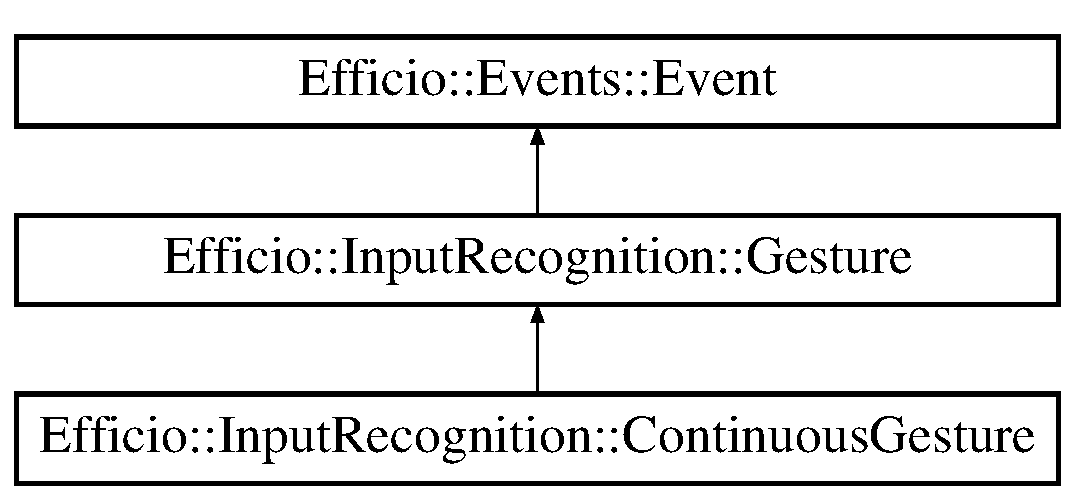
\includegraphics[height=3.000000cm]{class_efficio_1_1_input_recognition_1_1_continuous_gesture}
\end{center}
\end{figure}
\subsection*{Public Member Functions}
\begin{DoxyCompactItemize}
\item 
\hypertarget{class_efficio_1_1_input_recognition_1_1_continuous_gesture_aee0a3469492e3faed4dca28179645449}{}\label{class_efficio_1_1_input_recognition_1_1_continuous_gesture_aee0a3469492e3faed4dca28179645449} 
Gesture\+Type \hyperlink{class_efficio_1_1_input_recognition_1_1_continuous_gesture_aee0a3469492e3faed4dca28179645449}{Get\+Type} ()
\begin{DoxyCompactList}\small\item\em Gets the type of gesture that is occurring. \end{DoxyCompactList}\item 
\hypertarget{class_efficio_1_1_input_recognition_1_1_continuous_gesture_a29e6beed9d0f1745200412815974db7e}{}\label{class_efficio_1_1_input_recognition_1_1_continuous_gesture_a29e6beed9d0f1745200412815974db7e} 
virtual Gesture\+State \hyperlink{class_efficio_1_1_input_recognition_1_1_continuous_gesture_a29e6beed9d0f1745200412815974db7e}{Get\+Gesture\+State} ()=0
\begin{DoxyCompactList}\small\item\em Gets the state of the gesture. \end{DoxyCompactList}\end{DoxyCompactItemize}


\subsection{Detailed Description}
Continuous gestures are gestures that are done over time. 

The documentation for this class was generated from the following files\+:\begin{DoxyCompactItemize}
\item 
Continuous\+Gesture.\+h\item 
Continuous\+Gesture.\+cpp\end{DoxyCompactItemize}

\hypertarget{class_efficio_1_1_device}{}\section{Efficio\+:\+:Device Class Reference}
\label{class_efficio_1_1_device}\index{Efficio\+::\+Device@{Efficio\+::\+Device}}


Any device which can feel data into Efficio.  




{\ttfamily \#include $<$Device.\+h$>$}

Inheritance diagram for Efficio\+:\+:Device\+:\begin{figure}[H]
\begin{center}
\leavevmode
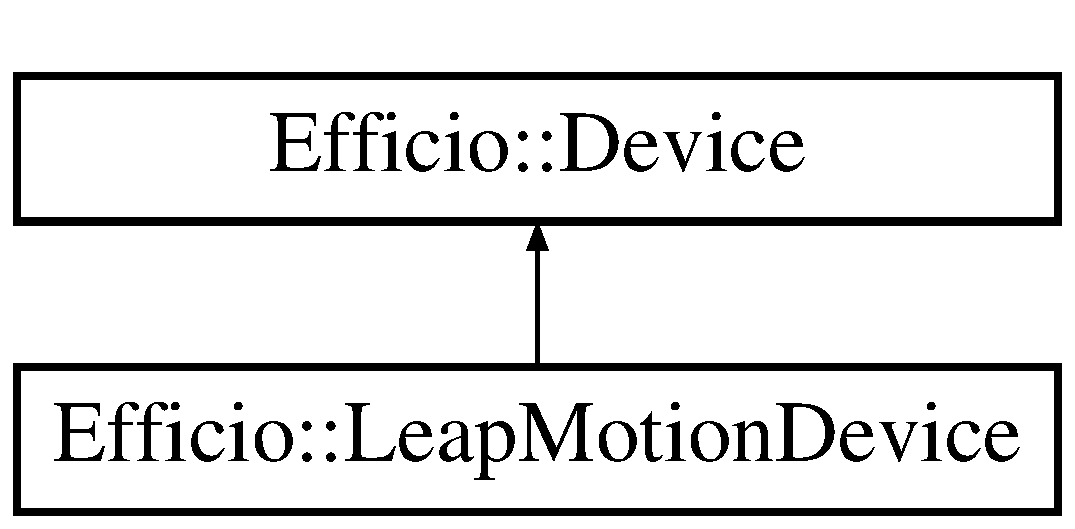
\includegraphics[height=2.000000cm]{class_efficio_1_1_device}
\end{center}
\end{figure}
\subsection*{Public Member Functions}
\begin{DoxyCompactItemize}
\item 
{\bfseries Device} (bool enabled=true)\hypertarget{class_efficio_1_1_device_a03b5d83501b593eced3d011954ca265f}{}\label{class_efficio_1_1_device_a03b5d83501b593eced3d011954ca265f}

\item 
bool \hyperlink{class_efficio_1_1_device_a51228fd0878a8514a28844a934a95625}{Connected} ()\hypertarget{class_efficio_1_1_device_a51228fd0878a8514a28844a934a95625}{}\label{class_efficio_1_1_device_a51228fd0878a8514a28844a934a95625}

\begin{DoxyCompactList}\small\item\em A Boolean indicating whether or nbot the device is connected and ready to feed data into Efficio. \end{DoxyCompactList}\item 
virtual Efficio\+::\+Device\+Status \hyperlink{class_efficio_1_1_device_a4fc83f754676de245976e1d1bb08b392}{Status} ()=0\hypertarget{class_efficio_1_1_device_a4fc83f754676de245976e1d1bb08b392}{}\label{class_efficio_1_1_device_a4fc83f754676de245976e1d1bb08b392}

\begin{DoxyCompactList}\small\item\em The status of the device. \end{DoxyCompactList}\item 
virtual Efficio\+::\+Tracking\+Type \hyperlink{class_efficio_1_1_device_ab655d0b6f140954de99fc4f187aca261}{Tracking\+Types} ()=0\hypertarget{class_efficio_1_1_device_ab655d0b6f140954de99fc4f187aca261}{}\label{class_efficio_1_1_device_ab655d0b6f140954de99fc4f187aca261}

\begin{DoxyCompactList}\small\item\em The type of data the device is able to track. \end{DoxyCompactList}\item 
virtual void \hyperlink{class_efficio_1_1_device_a852ea0bc779e5ec543b2a1162986ef7c}{Connect} ()=0\hypertarget{class_efficio_1_1_device_a852ea0bc779e5ec543b2a1162986ef7c}{}\label{class_efficio_1_1_device_a852ea0bc779e5ec543b2a1162986ef7c}

\begin{DoxyCompactList}\small\item\em Connects the device. \end{DoxyCompactList}\item 
virtual void \hyperlink{class_efficio_1_1_device_a8fb17a0b95255e8947cca9dcddcff26c}{Disconnect} ()=0\hypertarget{class_efficio_1_1_device_a8fb17a0b95255e8947cca9dcddcff26c}{}\label{class_efficio_1_1_device_a8fb17a0b95255e8947cca9dcddcff26c}

\begin{DoxyCompactList}\small\item\em Disconnects the device. \end{DoxyCompactList}\item 
virtual bool \hyperlink{class_efficio_1_1_device_a43eda953d99df9ee4df66df44c205773}{Has\+Frame} ()=0\hypertarget{class_efficio_1_1_device_a43eda953d99df9ee4df66df44c205773}{}\label{class_efficio_1_1_device_a43eda953d99df9ee4df66df44c205773}

\begin{DoxyCompactList}\small\item\em A Boolean indicating whether or not the device has a new frame for Efficio. \end{DoxyCompactList}\item 
virtual Leap\+::\+Frame \hyperlink{class_efficio_1_1_device_a82a46c74f3f75c9b2b08edbe6d2b5477}{Get\+Frame} ()=0\hypertarget{class_efficio_1_1_device_a82a46c74f3f75c9b2b08edbe6d2b5477}{}\label{class_efficio_1_1_device_a82a46c74f3f75c9b2b08edbe6d2b5477}

\begin{DoxyCompactList}\small\item\em Gets the current frame from the device. \end{DoxyCompactList}\end{DoxyCompactItemize}
\subsection*{Public Attributes}
\begin{DoxyCompactItemize}
\item 
std\+::string \hyperlink{class_efficio_1_1_device_ade0a5b10efa326ba8c4fdd9e37d89084}{ID}\hypertarget{class_efficio_1_1_device_ade0a5b10efa326ba8c4fdd9e37d89084}{}\label{class_efficio_1_1_device_ade0a5b10efa326ba8c4fdd9e37d89084}

\begin{DoxyCompactList}\small\item\em The unique ID of the device. \end{DoxyCompactList}\item 
\hyperlink{class_efficio_1_1_vector3}{Vector3} \hyperlink{class_efficio_1_1_device_a21ba05537c6978805f090e13c62ed220}{Position}\hypertarget{class_efficio_1_1_device_a21ba05537c6978805f090e13c62ed220}{}\label{class_efficio_1_1_device_a21ba05537c6978805f090e13c62ed220}

\begin{DoxyCompactList}\small\item\em The position of the device in the consuming application. \end{DoxyCompactList}\item 
\hyperlink{class_efficio_1_1_vector3}{Vector3} \hyperlink{class_efficio_1_1_device_a4da01030cb4382f23700edce87756b16}{Direction}\hypertarget{class_efficio_1_1_device_a4da01030cb4382f23700edce87756b16}{}\label{class_efficio_1_1_device_a4da01030cb4382f23700edce87756b16}

\begin{DoxyCompactList}\small\item\em The direction of the device in the consuming application. \end{DoxyCompactList}\item 
bool \hyperlink{class_efficio_1_1_device_ae724390ac1fadd47e528e0231bacf290}{Enabled}\hypertarget{class_efficio_1_1_device_ae724390ac1fadd47e528e0231bacf290}{}\label{class_efficio_1_1_device_ae724390ac1fadd47e528e0231bacf290}

\begin{DoxyCompactList}\small\item\em A Boolean indicating whether or not the device is enabled. \end{DoxyCompactList}\end{DoxyCompactItemize}


\subsection{Detailed Description}
Any device which can feel data into Efficio. 

The documentation for this class was generated from the following files\+:\begin{DoxyCompactItemize}
\item 
Device.\+h\item 
Device.\+cpp\end{DoxyCompactItemize}

\hypertarget{class_efficio_1_1_configuration_1_1_device_configuration}{}\section{Efficio\+:\+:Configuration\+:\+:Device\+Configuration Class Reference}
\label{class_efficio_1_1_configuration_1_1_device_configuration}\index{Efficio\+::\+Configuration\+::\+Device\+Configuration@{Efficio\+::\+Configuration\+::\+Device\+Configuration}}


The device configuration is used to configure the devices with which Efficio can work.  




{\ttfamily \#include $<$Device\+Configuration.\+h$>$}

\subsection*{Public Attributes}
\begin{DoxyCompactItemize}
\item 
\hyperlink{class_efficio_1_1_configuration_1_1_leap_configuration}{Leap\+Configuration} \hyperlink{class_efficio_1_1_configuration_1_1_device_configuration_aa5c43ffa75c5483880a21ef3490b54d6}{Leap\+Configuration}\hypertarget{class_efficio_1_1_configuration_1_1_device_configuration_aa5c43ffa75c5483880a21ef3490b54d6}{}\label{class_efficio_1_1_configuration_1_1_device_configuration_aa5c43ffa75c5483880a21ef3490b54d6}

\begin{DoxyCompactList}\small\item\em The configuration for the Leap Motion. \end{DoxyCompactList}\end{DoxyCompactItemize}


\subsection{Detailed Description}
The device configuration is used to configure the devices with which Efficio can work. 

The documentation for this class was generated from the following files\+:\begin{DoxyCompactItemize}
\item 
Device\+Configuration.\+h\item 
Device\+Configuration.\+cpp\end{DoxyCompactItemize}

\hypertarget{class_efficio_1_1_device_manager}{}\section{Efficio\+:\+:Device\+Manager Class Reference}
\label{class_efficio_1_1_device_manager}\index{Efficio\+::\+Device\+Manager@{Efficio\+::\+Device\+Manager}}


Manages all the devices connected to Efficio.  




{\ttfamily \#include $<$Device\+Manager.\+h$>$}

\subsection*{Public Member Functions}
\begin{DoxyCompactItemize}
\item 
void \hyperlink{class_efficio_1_1_device_manager_a4025caa83ba0dd4b4ba619654e4bf791}{Add\+Device} (std\+::shared\+\_\+ptr$<$ \hyperlink{class_efficio_1_1_device}{Efficio\+::\+Device} $>$ device)\hypertarget{class_efficio_1_1_device_manager_a4025caa83ba0dd4b4ba619654e4bf791}{}\label{class_efficio_1_1_device_manager_a4025caa83ba0dd4b4ba619654e4bf791}

\begin{DoxyCompactList}\small\item\em Adds a device to Efficio. \end{DoxyCompactList}\item 
std\+::vector$<$ std\+::shared\+\_\+ptr$<$ \hyperlink{class_efficio_1_1_device}{Efficio\+::\+Device} $>$ $>$ \hyperlink{class_efficio_1_1_device_manager_abed1c1e08d2fe7defef21fded68782b9}{Get\+Devices} ()\hypertarget{class_efficio_1_1_device_manager_abed1c1e08d2fe7defef21fded68782b9}{}\label{class_efficio_1_1_device_manager_abed1c1e08d2fe7defef21fded68782b9}

\begin{DoxyCompactList}\small\item\em Gets all the registered devices. \end{DoxyCompactList}\item 
std\+::vector$<$ std\+::shared\+\_\+ptr$<$ \hyperlink{class_efficio_1_1_device}{Efficio\+::\+Device} $>$ $>$ \hyperlink{class_efficio_1_1_device_manager_a21da4a9f44bc128e70115de8ab54bc4e}{Get\+Connected\+Devices} ()\hypertarget{class_efficio_1_1_device_manager_a21da4a9f44bc128e70115de8ab54bc4e}{}\label{class_efficio_1_1_device_manager_a21da4a9f44bc128e70115de8ab54bc4e}

\begin{DoxyCompactList}\small\item\em Gets all the connected devices. \end{DoxyCompactList}\item 
std\+::vector$<$ std\+::shared\+\_\+ptr$<$ \hyperlink{class_efficio_1_1_device}{Efficio\+::\+Device} $>$ $>$ \hyperlink{class_efficio_1_1_device_manager_a91a1c03cfe7f4268e9ed5ad0350b4a57}{Get\+Devices\+With\+Status} (Efficio\+::\+Device\+Status status)\hypertarget{class_efficio_1_1_device_manager_a91a1c03cfe7f4268e9ed5ad0350b4a57}{}\label{class_efficio_1_1_device_manager_a91a1c03cfe7f4268e9ed5ad0350b4a57}

\begin{DoxyCompactList}\small\item\em Gets all the devices with a matching status. \end{DoxyCompactList}\item 
std\+::shared\+\_\+ptr$<$ \hyperlink{class_efficio_1_1_device}{Efficio\+::\+Device} $>$ \hyperlink{class_efficio_1_1_device_manager_aeae743bb7d5d973f3245ae69d468befd}{Get\+Device\+By\+ID} (std\+::string ID)\hypertarget{class_efficio_1_1_device_manager_aeae743bb7d5d973f3245ae69d468befd}{}\label{class_efficio_1_1_device_manager_aeae743bb7d5d973f3245ae69d468befd}

\begin{DoxyCompactList}\small\item\em Gets a device by ID. \end{DoxyCompactList}\item 
void \hyperlink{class_efficio_1_1_device_manager_adaf266b0b68312621e331f2eb672c9cc}{Remove\+Device} (std\+::string ID)\hypertarget{class_efficio_1_1_device_manager_adaf266b0b68312621e331f2eb672c9cc}{}\label{class_efficio_1_1_device_manager_adaf266b0b68312621e331f2eb672c9cc}

\begin{DoxyCompactList}\small\item\em Removes a device by ID. \end{DoxyCompactList}\end{DoxyCompactItemize}


\subsection{Detailed Description}
Manages all the devices connected to Efficio. 

The documentation for this class was generated from the following files\+:\begin{DoxyCompactItemize}
\item 
Device\+Manager.\+h\item 
Device\+Manager.\+cpp\end{DoxyCompactItemize}

\hypertarget{class_efficio_1_1_input_recognition_1_1_discrete_gesture}{}\section{Efficio\+:\+:Input\+Recognition\+:\+:Discrete\+Gesture Class Reference}
\label{class_efficio_1_1_input_recognition_1_1_discrete_gesture}\index{Efficio\+::\+Input\+Recognition\+::\+Discrete\+Gesture@{Efficio\+::\+Input\+Recognition\+::\+Discrete\+Gesture}}


Discrete gestures are gestures that are always in a completed state.  




{\ttfamily \#include $<$Discrete\+Gesture.\+h$>$}

Inheritance diagram for Efficio\+:\+:Input\+Recognition\+:\+:Discrete\+Gesture\+:\begin{figure}[H]
\begin{center}
\leavevmode
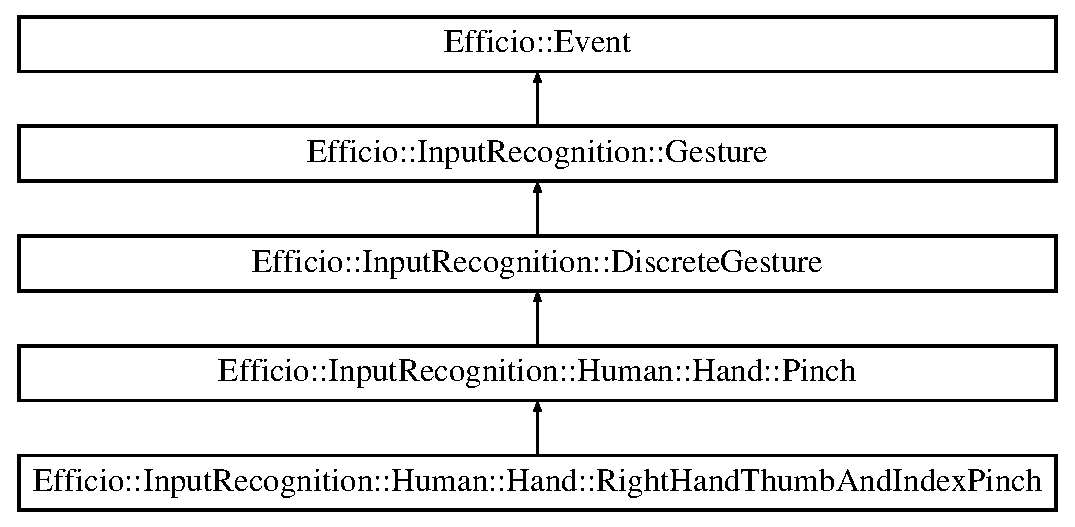
\includegraphics[height=4.000000cm]{class_efficio_1_1_input_recognition_1_1_discrete_gesture}
\end{center}
\end{figure}
\subsection*{Public Member Functions}
\begin{DoxyCompactItemize}
\item 
Gesture\+Type \hyperlink{class_efficio_1_1_input_recognition_1_1_discrete_gesture_aa41d3e90b680094da94183a1a1ed3b2a}{Get\+Type} ()\hypertarget{class_efficio_1_1_input_recognition_1_1_discrete_gesture_aa41d3e90b680094da94183a1a1ed3b2a}{}\label{class_efficio_1_1_input_recognition_1_1_discrete_gesture_aa41d3e90b680094da94183a1a1ed3b2a}

\begin{DoxyCompactList}\small\item\em Gets the type of gesture that is occurring. \end{DoxyCompactList}\item 
Gesture\+State \hyperlink{class_efficio_1_1_input_recognition_1_1_discrete_gesture_a18ff1c5231925c581ac3a6add9edfd67}{Get\+Gesture\+State} ()\hypertarget{class_efficio_1_1_input_recognition_1_1_discrete_gesture_a18ff1c5231925c581ac3a6add9edfd67}{}\label{class_efficio_1_1_input_recognition_1_1_discrete_gesture_a18ff1c5231925c581ac3a6add9edfd67}

\begin{DoxyCompactList}\small\item\em Gets the state of the gesture. \end{DoxyCompactList}\end{DoxyCompactItemize}


\subsection{Detailed Description}
Discrete gestures are gestures that are always in a completed state. 

The documentation for this class was generated from the following files\+:\begin{DoxyCompactItemize}
\item 
Discrete\+Gesture.\+h\item 
Discrete\+Gesture.\+cpp\end{DoxyCompactItemize}

\hypertarget{class_efficio_1_1_efficio_frame}{}\section{Efficio\+:\+:Efficio\+Frame Class Reference}
\label{class_efficio_1_1_efficio_frame}\index{Efficio\+::\+Efficio\+Frame@{Efficio\+::\+Efficio\+Frame}}


Object containing all processed and raw signals.  




{\ttfamily \#include $<$Efficio\+Frame.\+h$>$}

\subsection*{Public Member Functions}
\begin{DoxyCompactItemize}
\item 
{\bfseries Efficio\+Frame} (int ID)\hypertarget{class_efficio_1_1_efficio_frame_a9b49dc8882fa2c58ebcd8710bb14de91}{}\label{class_efficio_1_1_efficio_frame_a9b49dc8882fa2c58ebcd8710bb14de91}

\item 
std\+::vector$<$ std\+::shared\+\_\+ptr$<$ \hyperlink{class_efficio_1_1_events_1_1_event}{Efficio\+::\+Events\+::\+Event} $>$ $>$ {\bfseries Get\+Events} ()\hypertarget{class_efficio_1_1_efficio_frame_a219e88c37091c04515e7022c65300654}{}\label{class_efficio_1_1_efficio_frame_a219e88c37091c04515e7022c65300654}

\item 
std\+::vector$<$ std\+::shared\+\_\+ptr$<$ \hyperlink{class_efficio_1_1_models_1_1_human_1_1_hand}{Efficio\+::\+Models\+::\+Human\+::\+Hand} $>$ $>$ {\bfseries Get\+Hands} ()\hypertarget{class_efficio_1_1_efficio_frame_a2d6b1d6242890666e52a9d09bca6d610}{}\label{class_efficio_1_1_efficio_frame_a2d6b1d6242890666e52a9d09bca6d610}

\item 
void {\bfseries Add\+Event} (std\+::shared\+\_\+ptr$<$ \hyperlink{class_efficio_1_1_events_1_1_event}{Efficio\+::\+Events\+::\+Event} $>$ event\+Ptr)\hypertarget{class_efficio_1_1_efficio_frame_a2a50c673ea34e5d85707a55099ebae63}{}\label{class_efficio_1_1_efficio_frame_a2a50c673ea34e5d85707a55099ebae63}

\item 
void {\bfseries Add\+Hand} (std\+::shared\+\_\+ptr$<$ \hyperlink{class_efficio_1_1_models_1_1_human_1_1_hand}{Efficio\+::\+Models\+::\+Human\+::\+Hand} $>$ hand\+Ptr)\hypertarget{class_efficio_1_1_efficio_frame_aa8aba8a6ee0efc3194b9a9065b932fb2}{}\label{class_efficio_1_1_efficio_frame_aa8aba8a6ee0efc3194b9a9065b932fb2}

\end{DoxyCompactItemize}
\subsection*{Public Attributes}
\begin{DoxyCompactItemize}
\item 
int {\bfseries ID}\hypertarget{class_efficio_1_1_efficio_frame_aa994a72ec58afb3b6b64b9e05a9d0ba9}{}\label{class_efficio_1_1_efficio_frame_aa994a72ec58afb3b6b64b9e05a9d0ba9}

\end{DoxyCompactItemize}


\subsection{Detailed Description}
Object containing all processed and raw signals. 

The documentation for this class was generated from the following files\+:\begin{DoxyCompactItemize}
\item 
Efficio\+Frame.\+h\item 
Efficio\+Frame.\+cpp\end{DoxyCompactItemize}

\hypertarget{class_efficio_1_1_engine}{}\section{Efficio\+:\+:Engine Class Reference}
\label{class_efficio_1_1_engine}\index{Efficio\+::\+Engine@{Efficio\+::\+Engine}}


Efficio engine for retrieving processed frames.  




{\ttfamily \#include $<$Engine.\+h$>$}

\subsection*{Public Member Functions}
\begin{DoxyCompactItemize}
\item 
void {\bfseries Start} ()\hypertarget{class_efficio_1_1_engine_a3b6e5c963c14df6e902f72df6a521fd1}{}\label{class_efficio_1_1_engine_a3b6e5c963c14df6e902f72df6a521fd1}

\item 
std\+::shared\+\_\+ptr$<$ \hyperlink{class_efficio_1_1_efficio_frame}{Efficio\+::\+Efficio\+Frame} $>$ \hyperlink{class_efficio_1_1_engine_a4f46a611516d157a32005a860128f9dc}{Get\+Frame} ()
\item 
std\+::shared\+\_\+ptr$<$ \hyperlink{class_efficio_1_1_efficio_frame}{Efficio\+::\+Efficio\+Frame} $>$ \hyperlink{class_efficio_1_1_engine_a9f81b122b1c2f768110675a79a842117}{Get\+Frame} (int count)
\end{DoxyCompactItemize}
\subsection*{Public Attributes}
\begin{DoxyCompactItemize}
\item 
\hyperlink{class_efficio_1_1_configuration_1_1_device_configuration}{Efficio\+::\+Configuration\+::\+Device\+Configuration} \hyperlink{class_efficio_1_1_engine_afbaba10c9c508bdcc16625a2e51a6148}{Device\+Configuration}\hypertarget{class_efficio_1_1_engine_afbaba10c9c508bdcc16625a2e51a6148}{}\label{class_efficio_1_1_engine_afbaba10c9c508bdcc16625a2e51a6148}

\begin{DoxyCompactList}\small\item\em The device configuration for Efficio. \end{DoxyCompactList}\item 
\hyperlink{class_efficio_1_1_device_manager}{Efficio\+::\+Device\+Manager} \hyperlink{class_efficio_1_1_engine_a09180d13f06e554000ada9f10c62065c}{Device\+Manager}\hypertarget{class_efficio_1_1_engine_a09180d13f06e554000ada9f10c62065c}{}\label{class_efficio_1_1_engine_a09180d13f06e554000ada9f10c62065c}

\begin{DoxyCompactList}\small\item\em The \hyperlink{class_efficio_1_1_device}{Device} Manager. \end{DoxyCompactList}\end{DoxyCompactItemize}


\subsection{Detailed Description}
Efficio engine for retrieving processed frames. 

\subsection{Member Function Documentation}
\index{Efficio\+::\+Engine@{Efficio\+::\+Engine}!Get\+Frame@{Get\+Frame}}
\index{Get\+Frame@{Get\+Frame}!Efficio\+::\+Engine@{Efficio\+::\+Engine}}
\subsubsection[{\texorpdfstring{Get\+Frame()}{GetFrame()}}]{\setlength{\rightskip}{0pt plus 5cm}std\+::shared\+\_\+ptr$<$ {\bf Efficio\+::\+Efficio\+Frame} $>$ Efficio\+::\+Engine\+::\+Get\+Frame (
\begin{DoxyParamCaption}
{}
\end{DoxyParamCaption}
)}\hypertarget{class_efficio_1_1_engine_a4f46a611516d157a32005a860128f9dc}{}\label{class_efficio_1_1_engine_a4f46a611516d157a32005a860128f9dc}
Gets the current \hyperlink{class_efficio_1_1_efficio_frame}{frame} from the runtime. \begin{DoxyReturn}{Returns}
the current frame. 
\end{DoxyReturn}
\index{Efficio\+::\+Engine@{Efficio\+::\+Engine}!Get\+Frame@{Get\+Frame}}
\index{Get\+Frame@{Get\+Frame}!Efficio\+::\+Engine@{Efficio\+::\+Engine}}
\subsubsection[{\texorpdfstring{Get\+Frame(int count)}{GetFrame(int count)}}]{\setlength{\rightskip}{0pt plus 5cm}std\+::shared\+\_\+ptr$<$ {\bf Efficio\+::\+Efficio\+Frame} $>$ Efficio\+::\+Engine\+::\+Get\+Frame (
\begin{DoxyParamCaption}
\item[{int}]{count}
\end{DoxyParamCaption}
)}\hypertarget{class_efficio_1_1_engine_a9f81b122b1c2f768110675a79a842117}{}\label{class_efficio_1_1_engine_a9f81b122b1c2f768110675a79a842117}
Gets the historical \hyperlink{class_efficio_1_1_efficio_frame}{frame} from the runtime. \begin{DoxyReturn}{Returns}
the current frame. 
\end{DoxyReturn}


The documentation for this class was generated from the following files\+:\begin{DoxyCompactItemize}
\item 
Engine.\+h\item 
Engine.\+cpp\end{DoxyCompactItemize}

\hypertarget{class_efficio_1_1_events_1_1_event}{}\section{Efficio\+:\+:Events\+:\+:Event Class Reference}
\label{class_efficio_1_1_events_1_1_event}\index{Efficio\+::\+Events\+::\+Event@{Efficio\+::\+Events\+::\+Event}}


The abstract class for all events within the Efficio system. Events are raised when anything notable happens within the Efficio ecosystem.  




{\ttfamily \#include $<$Event.\+h$>$}

Inheritance diagram for Efficio\+:\+:Events\+:\+:Event\+:\begin{figure}[H]
\begin{center}
\leavevmode
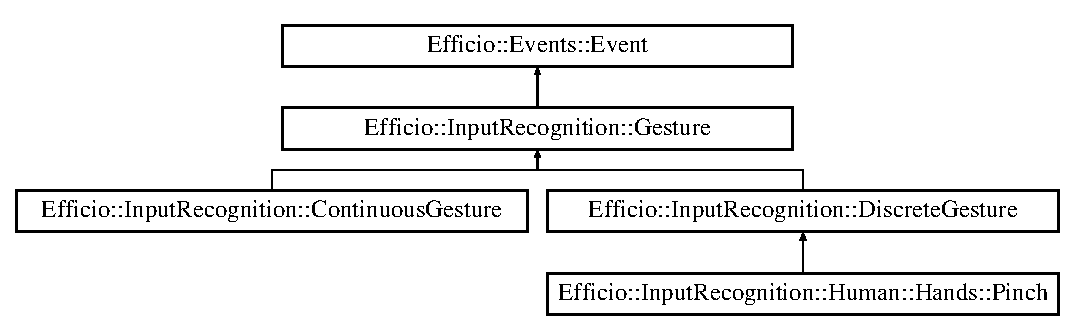
\includegraphics[height=4.000000cm]{class_efficio_1_1_events_1_1_event}
\end{center}
\end{figure}
\subsection*{Public Member Functions}
\begin{DoxyCompactItemize}
\item 
\hypertarget{class_efficio_1_1_events_1_1_event_a5758bd5812bfd09e0127892c490d553b}{}\label{class_efficio_1_1_events_1_1_event_a5758bd5812bfd09e0127892c490d553b} 
virtual Efficio\+::\+Events\+::\+Event\+Type {\bfseries Get\+Event\+Type} ()=0
\end{DoxyCompactItemize}


\subsection{Detailed Description}
The abstract class for all events within the Efficio system. Events are raised when anything notable happens within the Efficio ecosystem. 

The documentation for this class was generated from the following files\+:\begin{DoxyCompactItemize}
\item 
Event.\+h\item 
Event.\+cpp\end{DoxyCompactItemize}

\hypertarget{class_efficio_1_1_models_1_1_human_1_1_finger}{}\section{Efficio\+:\+:Models\+:\+:Human\+:\+:Finger Class Reference}
\label{class_efficio_1_1_models_1_1_human_1_1_finger}\index{Efficio\+::\+Models\+::\+Human\+::\+Finger@{Efficio\+::\+Models\+::\+Human\+::\+Finger}}
\subsection*{Public Member Functions}
\begin{DoxyCompactItemize}
\item 
{\bfseries Finger} (Finger\+Name finger\+Name, std\+::map$<$ Efficio\+::\+Models\+::\+Human\+::\+Joint\+Name, \hyperlink{class_efficio_1_1_vector3}{Efficio\+::\+Vector3} $>$ joint\+Positions)\hypertarget{class_efficio_1_1_models_1_1_human_1_1_finger_af50ea3b0f90fcb06b534fae022b4aa62}{}\label{class_efficio_1_1_models_1_1_human_1_1_finger_af50ea3b0f90fcb06b534fae022b4aa62}

\item 
\hyperlink{class_efficio_1_1_vector3}{Efficio\+::\+Vector3} {\bfseries Get\+Joint\+Position} (Efficio\+::\+Models\+::\+Human\+::\+Joint\+Name joint\+Name)\hypertarget{class_efficio_1_1_models_1_1_human_1_1_finger_a4c10fccb5ca87b762fe6752ec24d5052}{}\label{class_efficio_1_1_models_1_1_human_1_1_finger_a4c10fccb5ca87b762fe6752ec24d5052}

\end{DoxyCompactItemize}
\subsection*{Public Attributes}
\begin{DoxyCompactItemize}
\item 
Finger\+Name {\bfseries Name}\hypertarget{class_efficio_1_1_models_1_1_human_1_1_finger_ae73134fdf9c0ba485fce08abdf2e5e59}{}\label{class_efficio_1_1_models_1_1_human_1_1_finger_ae73134fdf9c0ba485fce08abdf2e5e59}

\end{DoxyCompactItemize}


The documentation for this class was generated from the following files\+:\begin{DoxyCompactItemize}
\item 
Finger.\+h\item 
Finger.\+cpp\end{DoxyCompactItemize}

\hypertarget{class_efficio_1_1_frame}{}\section{Efficio\+:\+:Frame Class Reference}
\label{class_efficio_1_1_frame}\index{Efficio\+::\+Frame@{Efficio\+::\+Frame}}
\subsection*{Public Member Functions}
\begin{DoxyCompactItemize}
\item 
\hyperlink{class_efficio_1_1_data_1_1_datum}{Efficio\+::\+Data\+::\+Datum} $\ast$ {\bfseries Get\+Data} (Efficio\+::\+Data\+::\+Datum\+Type data\+Type)\hypertarget{class_efficio_1_1_frame_a8e93ddb6f0dd2b69d56536f673bbc29c}{}\label{class_efficio_1_1_frame_a8e93ddb6f0dd2b69d56536f673bbc29c}

\item 
void {\bfseries Add\+Data} (\hyperlink{class_efficio_1_1_data_1_1_datum}{Efficio\+::\+Data\+::\+Datum} $\ast$datum)\hypertarget{class_efficio_1_1_frame_a75ccb8867d8acfe698073a67f33f72d4}{}\label{class_efficio_1_1_frame_a75ccb8867d8acfe698073a67f33f72d4}

\end{DoxyCompactItemize}
\subsection*{Public Attributes}
\begin{DoxyCompactItemize}
\item 
\hyperlink{class_efficio_1_1_hand_data}{Efficio\+::\+Hand\+Data} {\bfseries Hand\+Data}\hypertarget{class_efficio_1_1_frame_a546f841f8294491f08c83ef16e5b421c}{}\label{class_efficio_1_1_frame_a546f841f8294491f08c83ef16e5b421c}

\end{DoxyCompactItemize}


The documentation for this class was generated from the following files\+:\begin{DoxyCompactItemize}
\item 
Frame.\+h\item 
Frame.\+cpp\end{DoxyCompactItemize}

\hypertarget{class_efficio_1_1_input_recognition_1_1_gesture}{}\section{Efficio\+:\+:Input\+Recognition\+:\+:Gesture Class Reference}
\label{class_efficio_1_1_input_recognition_1_1_gesture}\index{Efficio\+::\+Input\+Recognition\+::\+Gesture@{Efficio\+::\+Input\+Recognition\+::\+Gesture}}


Base class for all gestures that may occur within the Efficio system.  




{\ttfamily \#include $<$Gesture.\+h$>$}

Inheritance diagram for Efficio\+:\+:Input\+Recognition\+:\+:Gesture\+:\begin{figure}[H]
\begin{center}
\leavevmode
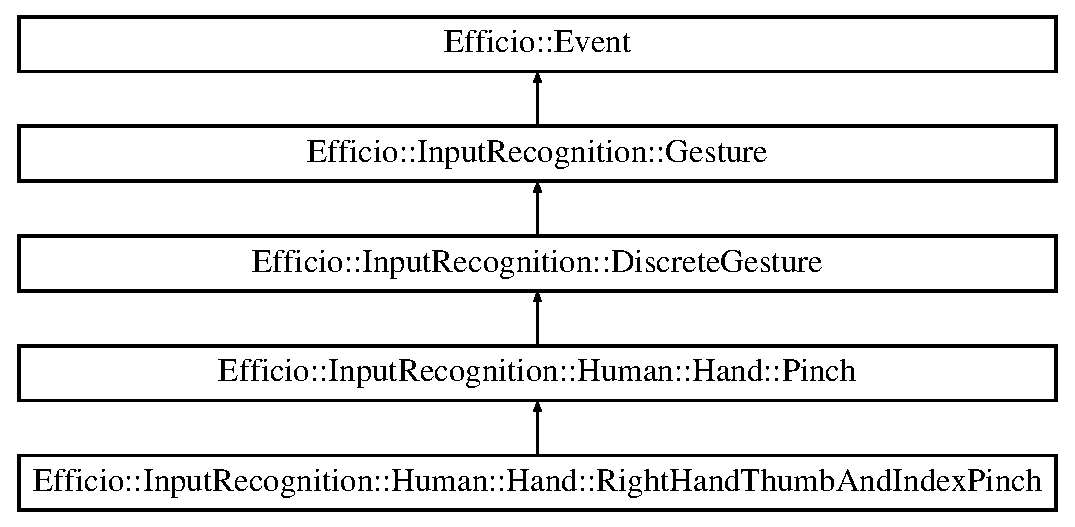
\includegraphics[height=4.000000cm]{class_efficio_1_1_input_recognition_1_1_gesture}
\end{center}
\end{figure}
\subsection*{Public Member Functions}
\begin{DoxyCompactItemize}
\item 
virtual Gesture\+Type \hyperlink{class_efficio_1_1_input_recognition_1_1_gesture_a751d03fe2bc9d025da065cec22936cd0}{Get\+Type} ()=0\hypertarget{class_efficio_1_1_input_recognition_1_1_gesture_a751d03fe2bc9d025da065cec22936cd0}{}\label{class_efficio_1_1_input_recognition_1_1_gesture_a751d03fe2bc9d025da065cec22936cd0}

\begin{DoxyCompactList}\small\item\em Gets the type of gesture that is occurring. \end{DoxyCompactList}\item 
virtual Gesture\+State \hyperlink{class_efficio_1_1_input_recognition_1_1_gesture_a0c607385ed5f969075f2e7a1eb11a85a}{Get\+Gesture\+State} ()=0\hypertarget{class_efficio_1_1_input_recognition_1_1_gesture_a0c607385ed5f969075f2e7a1eb11a85a}{}\label{class_efficio_1_1_input_recognition_1_1_gesture_a0c607385ed5f969075f2e7a1eb11a85a}

\begin{DoxyCompactList}\small\item\em Gets the state of the gesture. \end{DoxyCompactList}\item 
const std\+::time\+\_\+t \hyperlink{class_efficio_1_1_input_recognition_1_1_gesture_a22eb9d8533395b04d9f73b57afad09d6}{Get\+Start\+Time} ()\hypertarget{class_efficio_1_1_input_recognition_1_1_gesture_a22eb9d8533395b04d9f73b57afad09d6}{}\label{class_efficio_1_1_input_recognition_1_1_gesture_a22eb9d8533395b04d9f73b57afad09d6}

\begin{DoxyCompactList}\small\item\em Gets the start time of the gesture. \end{DoxyCompactList}\item 
const std\+::time\+\_\+t \hyperlink{class_efficio_1_1_input_recognition_1_1_gesture_a018fa00ce8db008e93fb988f649de9a6}{Get\+Gesture\+Duration} ()\hypertarget{class_efficio_1_1_input_recognition_1_1_gesture_a018fa00ce8db008e93fb988f649de9a6}{}\label{class_efficio_1_1_input_recognition_1_1_gesture_a018fa00ce8db008e93fb988f649de9a6}

\begin{DoxyCompactList}\small\item\em Getst the length of the gesture. \end{DoxyCompactList}\item 
virtual Efficio\+::\+Events\+::\+Event\+Type {\bfseries Get\+Event\+Type} ()=0\hypertarget{class_efficio_1_1_input_recognition_1_1_gesture_a2867983230c4bc6382e7b8e7e61215b6}{}\label{class_efficio_1_1_input_recognition_1_1_gesture_a2867983230c4bc6382e7b8e7e61215b6}

\end{DoxyCompactItemize}


\subsection{Detailed Description}
Base class for all gestures that may occur within the Efficio system. 

The documentation for this class was generated from the following files\+:\begin{DoxyCompactItemize}
\item 
Gesture.\+h\item 
Gesture.\+cpp\end{DoxyCompactItemize}

\hypertarget{class_efficio_1_1_models_1_1_human_1_1_hand}{}\section{Efficio\+:\+:Models\+:\+:Human\+:\+:Hand Class Reference}
\label{class_efficio_1_1_models_1_1_human_1_1_hand}\index{Efficio\+::\+Models\+::\+Human\+::\+Hand@{Efficio\+::\+Models\+::\+Human\+::\+Hand}}
\subsection*{Public Member Functions}
\begin{DoxyCompactItemize}
\item 
{\bfseries Hand} (std\+::vector$<$ \hyperlink{class_efficio_1_1_models_1_1_human_1_1_finger}{Efficio\+::\+Models\+::\+Human\+::\+Finger} $>$ fingers, Efficio\+::\+Body\+::\+Body\+Side side)\hypertarget{class_efficio_1_1_models_1_1_human_1_1_hand_a8917e801859dd364f255bbd38fa16762}{}\label{class_efficio_1_1_models_1_1_human_1_1_hand_a8917e801859dd364f255bbd38fa16762}

\end{DoxyCompactItemize}
\subsection*{Public Attributes}
\begin{DoxyCompactItemize}
\item 
std\+::vector$<$ \hyperlink{class_efficio_1_1_models_1_1_human_1_1_finger}{Efficio\+::\+Models\+::\+Human\+::\+Finger} $>$ {\bfseries Fingers}\hypertarget{class_efficio_1_1_models_1_1_human_1_1_hand_a96e7221f2a760f9c15a7ac935b538493}{}\label{class_efficio_1_1_models_1_1_human_1_1_hand_a96e7221f2a760f9c15a7ac935b538493}

\item 
Efficio\+::\+Body\+::\+Body\+Side {\bfseries Side}\hypertarget{class_efficio_1_1_models_1_1_human_1_1_hand_a9ead927dffc76db7a048cde9d3978c4d}{}\label{class_efficio_1_1_models_1_1_human_1_1_hand_a9ead927dffc76db7a048cde9d3978c4d}

\end{DoxyCompactItemize}


The documentation for this class was generated from the following files\+:\begin{DoxyCompactItemize}
\item 
Hand.\+h\item 
Hand.\+cpp\end{DoxyCompactItemize}

\hypertarget{class_efficio_1_1_hand_data}{}\section{Efficio\+:\+:Hand\+Data Class Reference}
\label{class_efficio_1_1_hand_data}\index{Efficio\+::\+Hand\+Data@{Efficio\+::\+Hand\+Data}}
\subsection*{Public Attributes}
\begin{DoxyCompactItemize}
\item 
std\+::vector$<$ \hyperlink{class_efficio_1_1_models_1_1_human_1_1_hand}{Efficio\+::\+Models\+::\+Human\+::\+Hand} $>$ {\bfseries Hands}\hypertarget{class_efficio_1_1_hand_data_a2c4c5e8dcb14692c918f1994859978f7}{}\label{class_efficio_1_1_hand_data_a2c4c5e8dcb14692c918f1994859978f7}

\end{DoxyCompactItemize}


The documentation for this class was generated from the following files\+:\begin{DoxyCompactItemize}
\item 
Hand\+Data.\+h\item 
Hand\+Data.\+cpp\end{DoxyCompactItemize}

\hypertarget{class_efficio_1_1_historical_frame_collection}{}\section{Efficio\+:\+:Historical\+Frame\+Collection Class Reference}
\label{class_efficio_1_1_historical_frame_collection}\index{Efficio\+::\+Historical\+Frame\+Collection@{Efficio\+::\+Historical\+Frame\+Collection}}


Collection of historical Efficio frames.  




{\ttfamily \#include $<$Historical\+Frame\+Collection.\+h$>$}

\subsection*{Public Member Functions}
\begin{DoxyCompactItemize}
\item 
\hypertarget{class_efficio_1_1_historical_frame_collection_a8bb93d37d7d634413626c52b5e8d1ea6}{}\label{class_efficio_1_1_historical_frame_collection_a8bb93d37d7d634413626c52b5e8d1ea6} 
void \hyperlink{class_efficio_1_1_historical_frame_collection_a8bb93d37d7d634413626c52b5e8d1ea6}{Add\+Frame} (std\+::shared\+\_\+ptr$<$ \hyperlink{class_efficio_1_1_efficio_frame}{Efficio\+::\+Efficio\+Frame} $>$ frame)
\begin{DoxyCompactList}\small\item\em Adds an Efficio frame to the history. \end{DoxyCompactList}\item 
\hypertarget{class_efficio_1_1_historical_frame_collection_abe5a246b4249f9596aae3cbcf04953b5}{}\label{class_efficio_1_1_historical_frame_collection_abe5a246b4249f9596aae3cbcf04953b5} 
std\+::shared\+\_\+ptr$<$ \hyperlink{class_efficio_1_1_efficio_frame}{Efficio\+::\+Efficio\+Frame} $>$ \hyperlink{class_efficio_1_1_historical_frame_collection_abe5a246b4249f9596aae3cbcf04953b5}{Get\+Frame} (int count\+Back)
\begin{DoxyCompactList}\small\item\em Gets a historical Efficio frame. \end{DoxyCompactList}\end{DoxyCompactItemize}


\subsection{Detailed Description}
Collection of historical Efficio frames. 

The documentation for this class was generated from the following files\+:\begin{DoxyCompactItemize}
\item 
Historical\+Frame\+Collection.\+h\item 
Historical\+Frame\+Collection.\+cpp\end{DoxyCompactItemize}

\hypertarget{class_efficio_1_1_models_1_1_human_1_1_joint}{}\section{Efficio\+:\+:Models\+:\+:Human\+:\+:Joint Class Reference}
\label{class_efficio_1_1_models_1_1_human_1_1_joint}\index{Efficio\+::\+Models\+::\+Human\+::\+Joint@{Efficio\+::\+Models\+::\+Human\+::\+Joint}}
\subsection*{Public Member Functions}
\begin{DoxyCompactItemize}
\item 
{\bfseries Joint} (Efficio\+::\+Models\+::\+Human\+::\+Joint\+Name name, \hyperlink{class_efficio_1_1_vector3}{Vector3} position)\hypertarget{class_efficio_1_1_models_1_1_human_1_1_joint_a2eab6b5945ddf7943f85a66a6d48ca6a}{}\label{class_efficio_1_1_models_1_1_human_1_1_joint_a2eab6b5945ddf7943f85a66a6d48ca6a}

\end{DoxyCompactItemize}
\subsection*{Public Attributes}
\begin{DoxyCompactItemize}
\item 
Joint\+Name {\bfseries Name}\hypertarget{class_efficio_1_1_models_1_1_human_1_1_joint_aa4fd209d1c5a00044ac4dd2648c64150}{}\label{class_efficio_1_1_models_1_1_human_1_1_joint_aa4fd209d1c5a00044ac4dd2648c64150}

\item 
\hyperlink{class_efficio_1_1_vector3}{Vector3} {\bfseries Position}\hypertarget{class_efficio_1_1_models_1_1_human_1_1_joint_a7d09e8e2be099d5400ef393ccc281ea0}{}\label{class_efficio_1_1_models_1_1_human_1_1_joint_a7d09e8e2be099d5400ef393ccc281ea0}

\end{DoxyCompactItemize}


The documentation for this class was generated from the following files\+:\begin{DoxyCompactItemize}
\item 
Joint.\+h\item 
Joint.\+cpp\end{DoxyCompactItemize}

\hypertarget{class_efficio_1_1_configuration_1_1_leap_configuration}{}\section{Efficio\+:\+:Configuration\+:\+:Leap\+Configuration Class Reference}
\label{class_efficio_1_1_configuration_1_1_leap_configuration}\index{Efficio\+::\+Configuration\+::\+Leap\+Configuration@{Efficio\+::\+Configuration\+::\+Leap\+Configuration}}
\subsection*{Public Attributes}
\begin{DoxyCompactItemize}
\item 
bool {\bfseries Enabled}\hypertarget{class_efficio_1_1_configuration_1_1_leap_configuration_a237eb567a1666e71d13e93bb2e9d86a9}{}\label{class_efficio_1_1_configuration_1_1_leap_configuration_a237eb567a1666e71d13e93bb2e9d86a9}

\end{DoxyCompactItemize}


The documentation for this class was generated from the following files\+:\begin{DoxyCompactItemize}
\item 
Leap\+Configuration.\+h\item 
Leap\+Configuration.\+cpp\end{DoxyCompactItemize}

\hypertarget{class_efficio_1_1_leap_motion_device}{}\section{Efficio\+:\+:Leap\+Motion\+Device Class Reference}
\label{class_efficio_1_1_leap_motion_device}\index{Efficio\+::\+Leap\+Motion\+Device@{Efficio\+::\+Leap\+Motion\+Device}}
Inheritance diagram for Efficio\+:\+:Leap\+Motion\+Device\+:\begin{figure}[H]
\begin{center}
\leavevmode
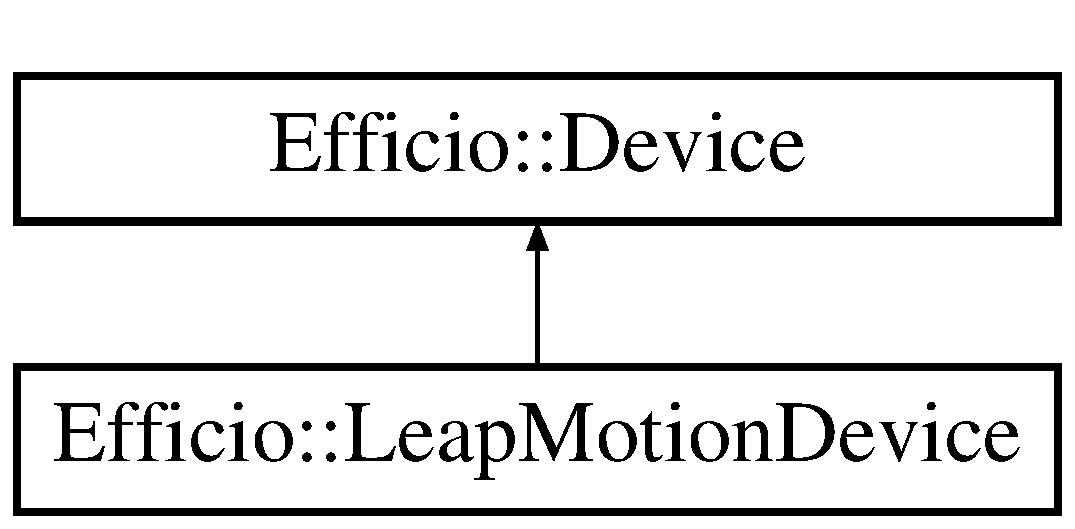
\includegraphics[height=2.000000cm]{class_efficio_1_1_leap_motion_device}
\end{center}
\end{figure}
\subsection*{Public Member Functions}
\begin{DoxyCompactItemize}
\item 
{\bfseries Leap\+Motion\+Device} (bool enabled=true)\hypertarget{class_efficio_1_1_leap_motion_device_a4c7db230fdb484f9b97ca95328e43f49}{}\label{class_efficio_1_1_leap_motion_device_a4c7db230fdb484f9b97ca95328e43f49}

\item 
Efficio\+::\+Device\+Status \hyperlink{class_efficio_1_1_leap_motion_device_aa8da27f1e5cbd65e88534f15df701914}{Status} ()\hypertarget{class_efficio_1_1_leap_motion_device_aa8da27f1e5cbd65e88534f15df701914}{}\label{class_efficio_1_1_leap_motion_device_aa8da27f1e5cbd65e88534f15df701914}

\begin{DoxyCompactList}\small\item\em The status of the device. \end{DoxyCompactList}\item 
Efficio\+::\+Tracking\+Type \hyperlink{class_efficio_1_1_leap_motion_device_a6234ba513473646dd7bf779d13e6c8ef}{Tracking\+Types} ()\hypertarget{class_efficio_1_1_leap_motion_device_a6234ba513473646dd7bf779d13e6c8ef}{}\label{class_efficio_1_1_leap_motion_device_a6234ba513473646dd7bf779d13e6c8ef}

\begin{DoxyCompactList}\small\item\em The type of data the device is able to track. \end{DoxyCompactList}\item 
void \hyperlink{class_efficio_1_1_leap_motion_device_a72bff092872814da4aec665b1fb09b5f}{Connect} ()\hypertarget{class_efficio_1_1_leap_motion_device_a72bff092872814da4aec665b1fb09b5f}{}\label{class_efficio_1_1_leap_motion_device_a72bff092872814da4aec665b1fb09b5f}

\begin{DoxyCompactList}\small\item\em Connects the device. \end{DoxyCompactList}\item 
void \hyperlink{class_efficio_1_1_leap_motion_device_aabe3f50f1a03994d5fd91d8aec615ff6}{Disconnect} ()\hypertarget{class_efficio_1_1_leap_motion_device_aabe3f50f1a03994d5fd91d8aec615ff6}{}\label{class_efficio_1_1_leap_motion_device_aabe3f50f1a03994d5fd91d8aec615ff6}

\begin{DoxyCompactList}\small\item\em Disconnects the device. \end{DoxyCompactList}\item 
bool \hyperlink{class_efficio_1_1_leap_motion_device_ad5a6c2c51426dd7544912d0d729984f6}{Has\+Frame} ()\hypertarget{class_efficio_1_1_leap_motion_device_ad5a6c2c51426dd7544912d0d729984f6}{}\label{class_efficio_1_1_leap_motion_device_ad5a6c2c51426dd7544912d0d729984f6}

\begin{DoxyCompactList}\small\item\em A Boolean indicating whether or not the device has a new frame for Efficio. \end{DoxyCompactList}\item 
\hyperlink{class_efficio_1_1_frame}{Efficio\+::\+Frame} \hyperlink{class_efficio_1_1_leap_motion_device_aebd0b9579f668aa92b0556e8b8687042}{Get\+Frame} ()\hypertarget{class_efficio_1_1_leap_motion_device_aebd0b9579f668aa92b0556e8b8687042}{}\label{class_efficio_1_1_leap_motion_device_aebd0b9579f668aa92b0556e8b8687042}

\begin{DoxyCompactList}\small\item\em Gets the current frame from the device. \end{DoxyCompactList}\end{DoxyCompactItemize}
\subsection*{Additional Inherited Members}


The documentation for this class was generated from the following files\+:\begin{DoxyCompactItemize}
\item 
Leap\+Motion\+Device.\+h\item 
Leap\+Motion\+Device.\+cpp\end{DoxyCompactItemize}

\hypertarget{class_efficio_1_1_input_recognition_1_1_human_1_1_hands_1_1_pinch}{}\section{Efficio\+:\+:Input\+Recognition\+:\+:Human\+:\+:Hands\+:\+:Pinch Class Reference}
\label{class_efficio_1_1_input_recognition_1_1_human_1_1_hands_1_1_pinch}\index{Efficio\+::\+Input\+Recognition\+::\+Human\+::\+Hands\+::\+Pinch@{Efficio\+::\+Input\+Recognition\+::\+Human\+::\+Hands\+::\+Pinch}}
Inheritance diagram for Efficio\+:\+:Input\+Recognition\+:\+:Human\+:\+:Hands\+:\+:Pinch\+:\begin{figure}[H]
\begin{center}
\leavevmode
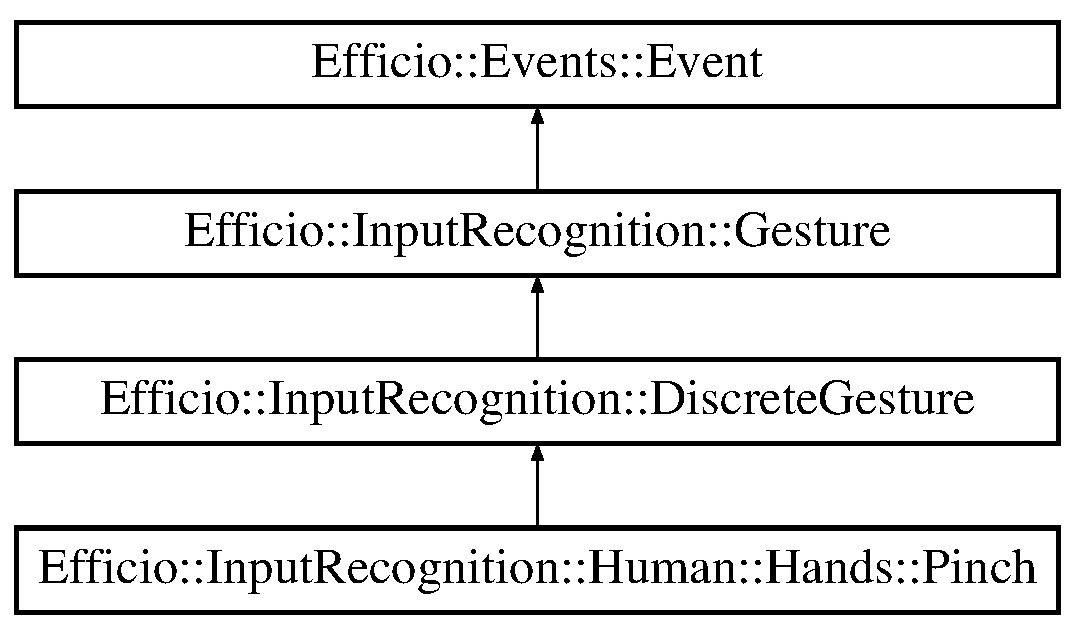
\includegraphics[height=4.000000cm]{class_efficio_1_1_input_recognition_1_1_human_1_1_hands_1_1_pinch}
\end{center}
\end{figure}
\subsection*{Public Member Functions}
\begin{DoxyCompactItemize}
\item 
{\bfseries Pinch} (Body\+::\+Body\+Side side, Body\+::\+Finger finger1, Body\+::\+Finger finger2, \hyperlink{class_efficio_1_1_vector3}{Vector3} position)\hypertarget{class_efficio_1_1_input_recognition_1_1_human_1_1_hands_1_1_pinch_a8471ee0196227f2c491925955449f534}{}\label{class_efficio_1_1_input_recognition_1_1_human_1_1_hands_1_1_pinch_a8471ee0196227f2c491925955449f534}

\item 
Efficio\+::\+Events\+::\+Event\+Type {\bfseries Get\+Event\+Type} ()\hypertarget{class_efficio_1_1_input_recognition_1_1_human_1_1_hands_1_1_pinch_a579897e092310066f9dab8df222fc863}{}\label{class_efficio_1_1_input_recognition_1_1_human_1_1_hands_1_1_pinch_a579897e092310066f9dab8df222fc863}

\end{DoxyCompactItemize}
\subsection*{Public Attributes}
\begin{DoxyCompactItemize}
\item 
\hyperlink{class_efficio_1_1_vector3}{Vector3} {\bfseries Position}\hypertarget{class_efficio_1_1_input_recognition_1_1_human_1_1_hands_1_1_pinch_aef25b5e89e91b9e9a7886a087c1b019f}{}\label{class_efficio_1_1_input_recognition_1_1_human_1_1_hands_1_1_pinch_aef25b5e89e91b9e9a7886a087c1b019f}

\item 
Body\+::\+Finger {\bfseries Finger1}\hypertarget{class_efficio_1_1_input_recognition_1_1_human_1_1_hands_1_1_pinch_ad8c959f5692cdf6e62381296c9d895fc}{}\label{class_efficio_1_1_input_recognition_1_1_human_1_1_hands_1_1_pinch_ad8c959f5692cdf6e62381296c9d895fc}

\item 
Body\+::\+Finger {\bfseries Finger2}\hypertarget{class_efficio_1_1_input_recognition_1_1_human_1_1_hands_1_1_pinch_a54b57c5b8ac5818d94a37fe52a5c2633}{}\label{class_efficio_1_1_input_recognition_1_1_human_1_1_hands_1_1_pinch_a54b57c5b8ac5818d94a37fe52a5c2633}

\item 
Body\+::\+Body\+Side {\bfseries Side}\hypertarget{class_efficio_1_1_input_recognition_1_1_human_1_1_hands_1_1_pinch_afacf4440ba63d00e52e205b0710798d1}{}\label{class_efficio_1_1_input_recognition_1_1_human_1_1_hands_1_1_pinch_afacf4440ba63d00e52e205b0710798d1}

\end{DoxyCompactItemize}


The documentation for this class was generated from the following files\+:\begin{DoxyCompactItemize}
\item 
Pinch.\+h\item 
Pinch.\+cpp\end{DoxyCompactItemize}

\hypertarget{class_efficio_1_1_input_recognition_1_1_human_1_1_hands_1_1_pinch_detector}{}\section{Efficio\+:\+:Input\+Recognition\+:\+:Human\+:\+:Hands\+:\+:Pinch\+Detector Class Reference}
\label{class_efficio_1_1_input_recognition_1_1_human_1_1_hands_1_1_pinch_detector}\index{Efficio\+::\+Input\+Recognition\+::\+Human\+::\+Hands\+::\+Pinch\+Detector@{Efficio\+::\+Input\+Recognition\+::\+Human\+::\+Hands\+::\+Pinch\+Detector}}
Inheritance diagram for Efficio\+:\+:Input\+Recognition\+:\+:Human\+:\+:Hands\+:\+:Pinch\+Detector\+:\begin{figure}[H]
\begin{center}
\leavevmode
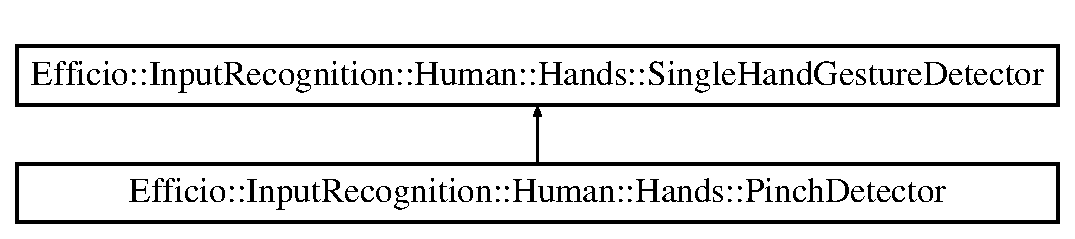
\includegraphics[height=2.000000cm]{class_efficio_1_1_input_recognition_1_1_human_1_1_hands_1_1_pinch_detector}
\end{center}
\end{figure}
\subsection*{Public Member Functions}
\begin{DoxyCompactItemize}
\item 
\hypertarget{class_efficio_1_1_input_recognition_1_1_human_1_1_hands_1_1_pinch_detector_a2488f7f3594f68d745da77364d025eef}{}\label{class_efficio_1_1_input_recognition_1_1_human_1_1_hands_1_1_pinch_detector_a2488f7f3594f68d745da77364d025eef} 
std\+::vector$<$ std\+::shared\+\_\+ptr$<$ \hyperlink{class_efficio_1_1_input_recognition_1_1_gesture}{Efficio\+::\+Input\+Recognition\+::\+Gesture} $>$ $>$ {\bfseries Detect} (Leap\+::\+Hand hand)
\end{DoxyCompactItemize}
\subsection*{Public Attributes}
\begin{DoxyCompactItemize}
\item 
\hypertarget{class_efficio_1_1_input_recognition_1_1_human_1_1_hands_1_1_pinch_detector_ace7cbaf0cc98103be15dfdc621a49f3f}{}\label{class_efficio_1_1_input_recognition_1_1_human_1_1_hands_1_1_pinch_detector_ace7cbaf0cc98103be15dfdc621a49f3f} 
bool {\bfseries Enabled}
\end{DoxyCompactItemize}
\subsection*{Additional Inherited Members}


The documentation for this class was generated from the following files\+:\begin{DoxyCompactItemize}
\item 
Pinch\+Detector.\+h\item 
Pinch\+Detector.\+cpp\end{DoxyCompactItemize}

\hypertarget{class_efficio_1_1_input_recognition_1_1_human_1_1_hands_1_1_single_hand_gesture}{}\section{Efficio\+:\+:Input\+Recognition\+:\+:Human\+:\+:Hands\+:\+:Single\+Hand\+Gesture Class Reference}
\label{class_efficio_1_1_input_recognition_1_1_human_1_1_hands_1_1_single_hand_gesture}\index{Efficio\+::\+Input\+Recognition\+::\+Human\+::\+Hands\+::\+Single\+Hand\+Gesture@{Efficio\+::\+Input\+Recognition\+::\+Human\+::\+Hands\+::\+Single\+Hand\+Gesture}}
Inheritance diagram for Efficio\+:\+:Input\+Recognition\+:\+:Human\+:\+:Hands\+:\+:Single\+Hand\+Gesture\+:\begin{figure}[H]
\begin{center}
\leavevmode
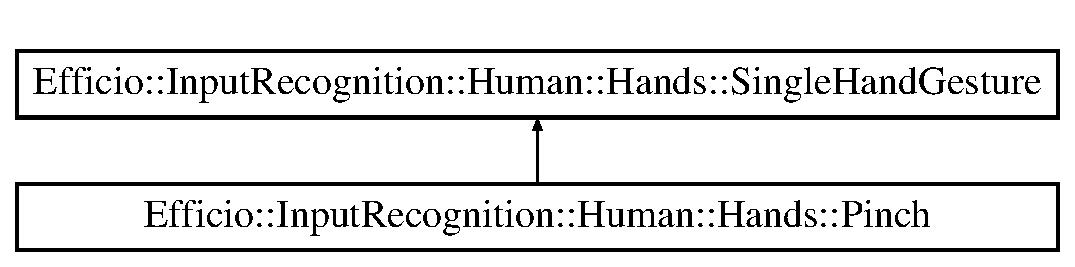
\includegraphics[height=2.000000cm]{class_efficio_1_1_input_recognition_1_1_human_1_1_hands_1_1_single_hand_gesture}
\end{center}
\end{figure}
\subsection*{Public Member Functions}
\begin{DoxyCompactItemize}
\item 
{\bfseries Single\+Hand\+Gesture} (Body\+::\+Body\+Side side)\hypertarget{class_efficio_1_1_input_recognition_1_1_human_1_1_hands_1_1_single_hand_gesture_a63a8fc2546dc1a7e5962eb09de469f34}{}\label{class_efficio_1_1_input_recognition_1_1_human_1_1_hands_1_1_single_hand_gesture_a63a8fc2546dc1a7e5962eb09de469f34}

\end{DoxyCompactItemize}
\subsection*{Public Attributes}
\begin{DoxyCompactItemize}
\item 
Body\+::\+Body\+Side {\bfseries Side}\hypertarget{class_efficio_1_1_input_recognition_1_1_human_1_1_hands_1_1_single_hand_gesture_ad46d8585b784c4e9c4425e813fab2d5b}{}\label{class_efficio_1_1_input_recognition_1_1_human_1_1_hands_1_1_single_hand_gesture_ad46d8585b784c4e9c4425e813fab2d5b}

\end{DoxyCompactItemize}


The documentation for this class was generated from the following files\+:\begin{DoxyCompactItemize}
\item 
Single\+Hand\+Gesture.\+h\item 
Single\+Hand\+Gesture.\+cpp\end{DoxyCompactItemize}

\hypertarget{class_efficio_1_1_input_recognition_1_1_human_1_1_hands_1_1_single_hand_gesture_detector}{}\section{Efficio\+:\+:Input\+Recognition\+:\+:Human\+:\+:Hands\+:\+:Single\+Hand\+Gesture\+Detector Class Reference}
\label{class_efficio_1_1_input_recognition_1_1_human_1_1_hands_1_1_single_hand_gesture_detector}\index{Efficio\+::\+Input\+Recognition\+::\+Human\+::\+Hands\+::\+Single\+Hand\+Gesture\+Detector@{Efficio\+::\+Input\+Recognition\+::\+Human\+::\+Hands\+::\+Single\+Hand\+Gesture\+Detector}}
\subsection*{Public Member Functions}
\begin{DoxyCompactItemize}
\item 
virtual std\+::vector$<$ std\+::shared\+\_\+ptr$<$ \hyperlink{class_efficio_1_1_input_recognition_1_1_gesture}{Efficio\+::\+Input\+Recognition\+::\+Gesture} $>$ $>$ {\bfseries Detect} (Leap\+::\+Hand hand)=0\hypertarget{class_efficio_1_1_input_recognition_1_1_human_1_1_hands_1_1_single_hand_gesture_detector_a6fb83b598c1f11539f6c49495c987994}{}\label{class_efficio_1_1_input_recognition_1_1_human_1_1_hands_1_1_single_hand_gesture_detector_a6fb83b598c1f11539f6c49495c987994}

\end{DoxyCompactItemize}
\subsection*{Protected Attributes}
\begin{DoxyCompactItemize}
\item 
std\+::array$<$ Efficio\+::\+Body\+::\+Finger\+Type, 5 $>$ {\bfseries Finger\+Names}
\end{DoxyCompactItemize}


\subsection{Member Data Documentation}
\index{Efficio\+::\+Input\+Recognition\+::\+Human\+::\+Hands\+::\+Single\+Hand\+Gesture\+Detector@{Efficio\+::\+Input\+Recognition\+::\+Human\+::\+Hands\+::\+Single\+Hand\+Gesture\+Detector}!Finger\+Names@{Finger\+Names}}
\index{Finger\+Names@{Finger\+Names}!Efficio\+::\+Input\+Recognition\+::\+Human\+::\+Hands\+::\+Single\+Hand\+Gesture\+Detector@{Efficio\+::\+Input\+Recognition\+::\+Human\+::\+Hands\+::\+Single\+Hand\+Gesture\+Detector}}
\subsubsection[{\texorpdfstring{Finger\+Names}{FingerNames}}]{\setlength{\rightskip}{0pt plus 5cm}std\+::array$<$Efficio\+::\+Body\+::\+Finger\+Type, 5$>$ Efficio\+::\+Input\+Recognition\+::\+Human\+::\+Hands\+::\+Single\+Hand\+Gesture\+Detector\+::\+Finger\+Names\hspace{0.3cm}{\ttfamily [protected]}}\hypertarget{class_efficio_1_1_input_recognition_1_1_human_1_1_hands_1_1_single_hand_gesture_detector_a500f4eb83fd6ba19b35622f4c510cb4a}{}\label{class_efficio_1_1_input_recognition_1_1_human_1_1_hands_1_1_single_hand_gesture_detector_a500f4eb83fd6ba19b35622f4c510cb4a}
{\bfseries Initial value\+:}
\begin{DoxyCode}
= 
                    \{ 
                        Efficio::Body::FingerType::Thumb,
                        Efficio::Body::FingerType::Index,
                        Efficio::Body::FingerType::Middle,
                        Efficio::Body::FingerType::Ring,
                        Efficio::Body::FingerType::Pinky
                    \}
\end{DoxyCode}


The documentation for this class was generated from the following file\+:\begin{DoxyCompactItemize}
\item 
Single\+Hand\+Gesture\+Detector.\+h\end{DoxyCompactItemize}

\hypertarget{struct_s_w_i_g___java_exceptions__t}{}\section{S\+W\+I\+G\+\_\+\+Java\+Exceptions\+\_\+t Struct Reference}
\label{struct_s_w_i_g___java_exceptions__t}\index{S\+W\+I\+G\+\_\+\+Java\+Exceptions\+\_\+t@{S\+W\+I\+G\+\_\+\+Java\+Exceptions\+\_\+t}}
\subsection*{Public Attributes}
\begin{DoxyCompactItemize}
\item 
S\+W\+I\+G\+\_\+\+Java\+Exception\+Codes {\bfseries code}\hypertarget{struct_s_w_i_g___java_exceptions__t_a04044dfc89f07ed39fe7bbb23f120d5a}{}\label{struct_s_w_i_g___java_exceptions__t_a04044dfc89f07ed39fe7bbb23f120d5a}

\item 
const char $\ast$ {\bfseries java\+\_\+exception}\hypertarget{struct_s_w_i_g___java_exceptions__t_a38dd5a9090f6d6c09f43d85536bc3154}{}\label{struct_s_w_i_g___java_exceptions__t_a38dd5a9090f6d6c09f43d85536bc3154}

\end{DoxyCompactItemize}


The documentation for this struct was generated from the following file\+:\begin{DoxyCompactItemize}
\item 
Runtime\+Java\+\_\+wrap.\+cxx\end{DoxyCompactItemize}

\hypertarget{struct_s_w_i_g__null__deleter}{}\section{S\+W\+I\+G\+\_\+null\+\_\+deleter Struct Reference}
\label{struct_s_w_i_g__null__deleter}\index{S\+W\+I\+G\+\_\+null\+\_\+deleter@{S\+W\+I\+G\+\_\+null\+\_\+deleter}}
\subsection*{Public Member Functions}
\begin{DoxyCompactItemize}
\item 
void {\bfseries operator()} (void const $\ast$) const \hypertarget{struct_s_w_i_g__null__deleter_aa95dacef916da5f0a455c37edaf8aefc}{}\label{struct_s_w_i_g__null__deleter_aa95dacef916da5f0a455c37edaf8aefc}

\end{DoxyCompactItemize}


The documentation for this struct was generated from the following file\+:\begin{DoxyCompactItemize}
\item 
Runtime\+Java\+\_\+wrap.\+cxx\end{DoxyCompactItemize}

\hypertarget{class_efficio_1_1_vector3}{}\section{Efficio\+:\+:Vector3 Class Reference}
\label{class_efficio_1_1_vector3}\index{Efficio\+::\+Vector3@{Efficio\+::\+Vector3}}
\subsection*{Public Member Functions}
\begin{DoxyCompactItemize}
\item 
{\bfseries Vector3} (float x, float y, float z)\hypertarget{class_efficio_1_1_vector3_a25ddecf52b20f83dad77f70f5fe856d7}{}\label{class_efficio_1_1_vector3_a25ddecf52b20f83dad77f70f5fe856d7}

\item 
float {\bfseries Distance\+To} (\hyperlink{class_efficio_1_1_vector3}{Efficio\+::\+Vector3} vector2)\hypertarget{class_efficio_1_1_vector3_ae819761f590d1f73677206aeb5933f50}{}\label{class_efficio_1_1_vector3_ae819761f590d1f73677206aeb5933f50}

\item 
float {\bfseries X} ()\hypertarget{class_efficio_1_1_vector3_a64c3100486b0bb40756a2ab871ec571a}{}\label{class_efficio_1_1_vector3_a64c3100486b0bb40756a2ab871ec571a}

\item 
float {\bfseries Y} ()\hypertarget{class_efficio_1_1_vector3_a2a49ce0090a5505d92c6cefa84afab5e}{}\label{class_efficio_1_1_vector3_a2a49ce0090a5505d92c6cefa84afab5e}

\item 
float {\bfseries Z} ()\hypertarget{class_efficio_1_1_vector3_ab2befc75a1b0c356ac23dd2ae9ef7041}{}\label{class_efficio_1_1_vector3_ab2befc75a1b0c356ac23dd2ae9ef7041}

\end{DoxyCompactItemize}


The documentation for this class was generated from the following files\+:\begin{DoxyCompactItemize}
\item 
Vector3.\+h\item 
Vector3.\+cpp\end{DoxyCompactItemize}

%--- End generated contents ---

% Index
\backmatter
\newpage
\phantomsection
\clearemptydoublepage
\addcontentsline{toc}{chapter}{Index}
\printindex

\end{document}
